\begin{figure}
\centering
\includegraphics[width=\textwidth,height=\textheight,keepaspectratio]{Figure_1.pdf}
\caption{CAT pipeline schematic}
The CAT pipeline takes as input a HAL alignment file, an existing annotation set and aligned RNA-seq reads. CAT uses the Cactus alignment to project annotations to other genomes using transMap  \citep{stanke2008using}. These transcript projections are then filtered and paralog resolved. Optionally, AUGUSTUS can be run into up to four parameterizations. All transcripts are classified for extrinsic support and structure and a ‘chooser’ algorithm picks the best representative for each input transcript, incorporating \textit{ab-initio} transcripts when they provide novel supported information. The final consensus gene set as well as associated feature tracks are used to create a assembly hub ready to be loaded by the UCSC Genome Browser. See Supplementary Figure \ref{supp_fig:pipeline} and Supplementary Note 1 for more detail.
\label{fig:pipeline}
\end{figure}


\begin{figure}
\centering
\includegraphics[width=0.8\textwidth,height=0.8\textheight,keepaspectratio]{Figure_2.pdf}
\caption{Primate annotation}
A) Validating CAT annotations using Iso-Seq data. As a baseline comparison, Iso-Seq data from human iPSCs were compared to the GENCODE V27 annotation. Iso-Seq data from chimpanzee, gorilla and orangutan iPSC lines were compared to respective species-specific annotations. The Iso-Seq data were clustered with ICE and collapsed using ToFU \citep{gordon2015widespread}. CAT annotation of PacBio great apes showed similar isoform concordance to human, and improvement over the older assemblies. B) Kallisto \citep{bray2015near} was used to quantify liver Illumina RNA-seq from each species on both the gene and transcript level on the existing and new great ape assemblies. Solid bars are transcripts or genes with transcripts per million (TPM) \textgreater 0.1, while shaded hatched bars are the remainder of the annotation sets. CAT annotation of great apes shows nearly the same number of expressed genes and isoforms as the GENCODE reference on human with the exception of orangutan. C) The number of novel isoforms and paralogous genes with Iso-Seq support discovered by analysis of AugustusPB and AugustusCGP predictions for each species. D) Kallisto protein-coding gene-level expression for chimpanzee iPSC RNA-seq is compared to human across all of the chimpanzee annotation and assembly combinations as well as when mapped directly to human. In all cases the x-axis is the TPM of human iPSC data mapped to human. The highest correlation (Pearson r=0.96) is seen when comparing Clint annotated with CAT to GRCh38 annotated with GENCODE V27.
\label{fig:primate}
\end{figure}


\begin{figure}
\centering
\includegraphics[width=\textwidth,height=0.75\textheight,keepaspectratio]{Figure_3.pdf}
\caption{Pseudo-diploid human annotation metrics}
A) The number and fraction of genes comparatively annotated from GENCODE V27 in each assembly. GENCODE biotypes are simplified into protein coding, lncRNA, ncRNA, pseudogene and other. Other includes processed transcripts, nonsense-mediated decay, and immune-related genes. B) Frame-shifting insertions, deletions and multiple of 3 indels that do not shift frame are reported for each assembly. Consistent with the great ape genomes, there is a systematic over-representation of coding deletions in Falcon assemblies, despite these assemblies coming from haploid cell lines. 10x Supernova assemblies also exhibit similar properties. C) Split gene analysis reports how often paralog-resolved transcript projections end up on different contigs, which can measure assembly gene-level contiguity. PacBio assemblies, especially CHM1, are the most contiguous.
\label{fig:human_metrics}
\end{figure}

\begin{figure}
\centering
\includegraphics[width=\textwidth,height=0.75\textheight,keepaspectratio]{Figure_4.pdf}
\caption{Pseudo-diploid human annotation examples}
A) UCSC Assembly Hub \citep{nguyen2014comparative} showing \textit{TRIB3} deletion in CHM1. Analysis of genes found in one genome and not the other led to the discovery of a novel structural variant specific to CHM1, which disables the gene \textit{TRIB3}. Spanning reads were found in both PacBio and Illumina whole-genome sequencing that validate the deletion. B) An example insertion near an exon of \textit{TAOK3} seen in one haplotype of NA12878. It was not possible to determine if this insertion effected transcription of this gene.
\label{fig:human_example}
\end{figure}


\begin{figure}
\centering
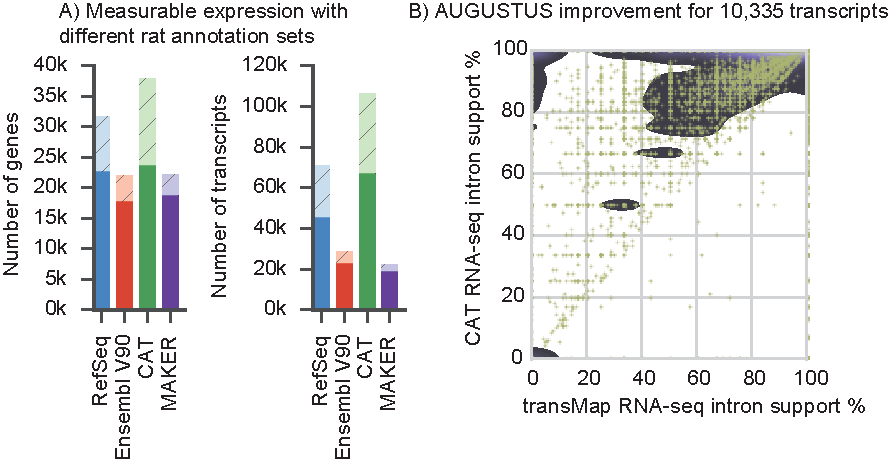
\includegraphics[width=\textwidth,height=\textheight,keepaspectratio]{Figure_5.pdf}
\caption{Validation of CAT annotation using rat}
A) Each transcript set was used to construct a Kallisto  \citep{bray2015near} index, and then all of the input RNA-seq for annotation were quantified. Solid bars are genes or transcripts with non-zero expression (TPM\textgreater 0.1) estimates, while light hatched bars are the remainder of the annotation set. CAT provides an annotation set with slightly more detectable genes than other annotation methods, and far more detectable isoforms. B) AugustusTMR provides a mechanism to clean up transcript projections and shift splice sites, fixing alignment errors as well as real evolutionary changes. Most of the 9,532 AugustusTMR transcripts chosen in consensus finding show an improvement in RNA-seq support, which is one of the features used in consensus finding.
\label{fig:rat_validation}
\end{figure}

\begin{figure}
\centering
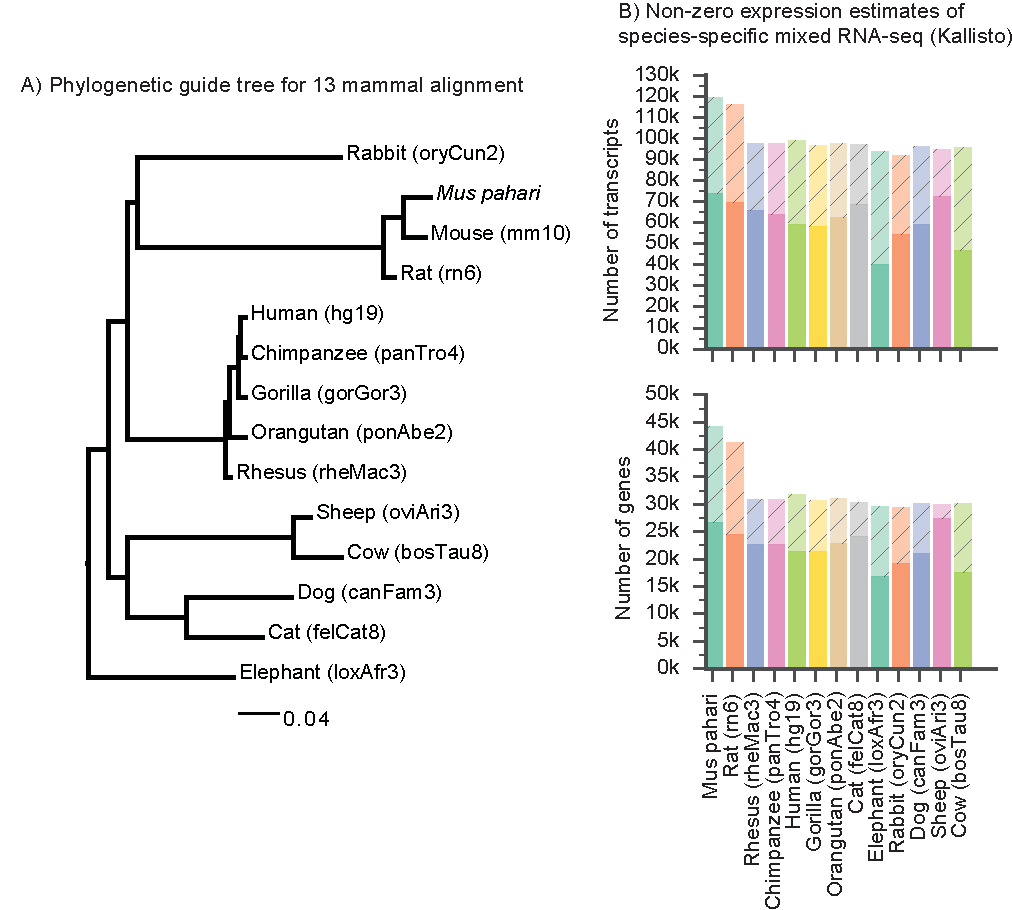
\includegraphics[width=0.7\textwidth,height=0.7\textheight,keepaspectratio]{Figure_6.pdf}
\caption{13-way annotation}
A) The phylogenetic guide tree for the 14-way mammal alignment. See the methods section for the exact Newick format tree. B) The gene annotation sets for each of the 13 mammalian genomes were quantified against the mixed input RNA-seq sets obtained from SRA. Genes or transcripts with TPM\textgreater 0.1 are solid colors, while genes or transcripts with no measurable expression are shaded. An average of 2.8 isoforms per gene per genome had quantifiable expression, suggesting that CAT can infer isoform information across long branch lengths.
\label{fig:13way}
\end{figure}

\begin{table}
\centering
A) Precision and recall in CAT annotation of rat\\
\begin{tabular}{|c|c|c|c|c|} \hline
Annotation & Exon precision & Exon recall & Intron precision & Intron recall \\ \hline
CAT & 0.703 & 0.559 & 0.861 & 0.734 \\ \hline
MAKER & 0.507 & 0.582 & 0.610 & 0.746 \\ \hline
\end{tabular}

\vspace{5mm}
B) Jaccard Similarity in rat annotation sets \\
\begin{tabular}{|c|c|c|} \hline
Annotation pair & Exon Jaccard similarity & Intron Jaccard similarity \\ \hline
EnsemblV90/RefSeq & 0.658 & 0.749 \\ \hline
CAT/EnsemblV90 & 0.649 & 0.740 \\ \hline
CAT/RefSeq & 0.648 & 0.841 \\ \hline
EnsemblV90/MAKER & 0.514 & 0.364 \\ \hline
CAT/MAKER & 0.484 & 0.334 \\ \hline
MAKER/RefSeq & 0.464 & 0.337 \\ \hline
\end{tabular}
\caption{Rat annotation similarity metrics}
A) Precision is the number of coding exons or coding introns that exactly match divided by the number of exons or introns in the Ensembl annotation, while recall is the number that exactly match divided by the number of exons or introns in the CAT or, respectively, MAKER annotation. B) Jaccard similarity of CDS introns and exons between rat annotation sets shows high similarity between CAT and existing Ensembl and RefSeq annotations, comparable to the similarity between Ensembl and RefSeq themselves.
\label{table:rat_similarity}
\end{table}

\begin{table}
\centering
\begin{tabular}{|c|c|c|c|c|c|} \hline
Exon precision & Exon recall & Intron precision & Intron recall & Isoform precision & Isoform recall \\ \hline
0.532 & 0.688 & 0.777 & 0.912 & 0.408 & 0.752 \\ \hline
\end{tabular}
\vspace{5mm}

\caption{Precision and recall of CAT annotation of hg19 using mouse isoforms}
Precision and recall are measured by looking at exact matches of coding introns, exons and isoforms. Isoforms are compared on a coding intron chain level. Precision and recall are defined in the same way as in Table \ref{table:rat_similarity}.
\label{table:validation}
\end{table}

\null\newpage